
\begin{figure*}[htb!]%[H]
\begin{center}
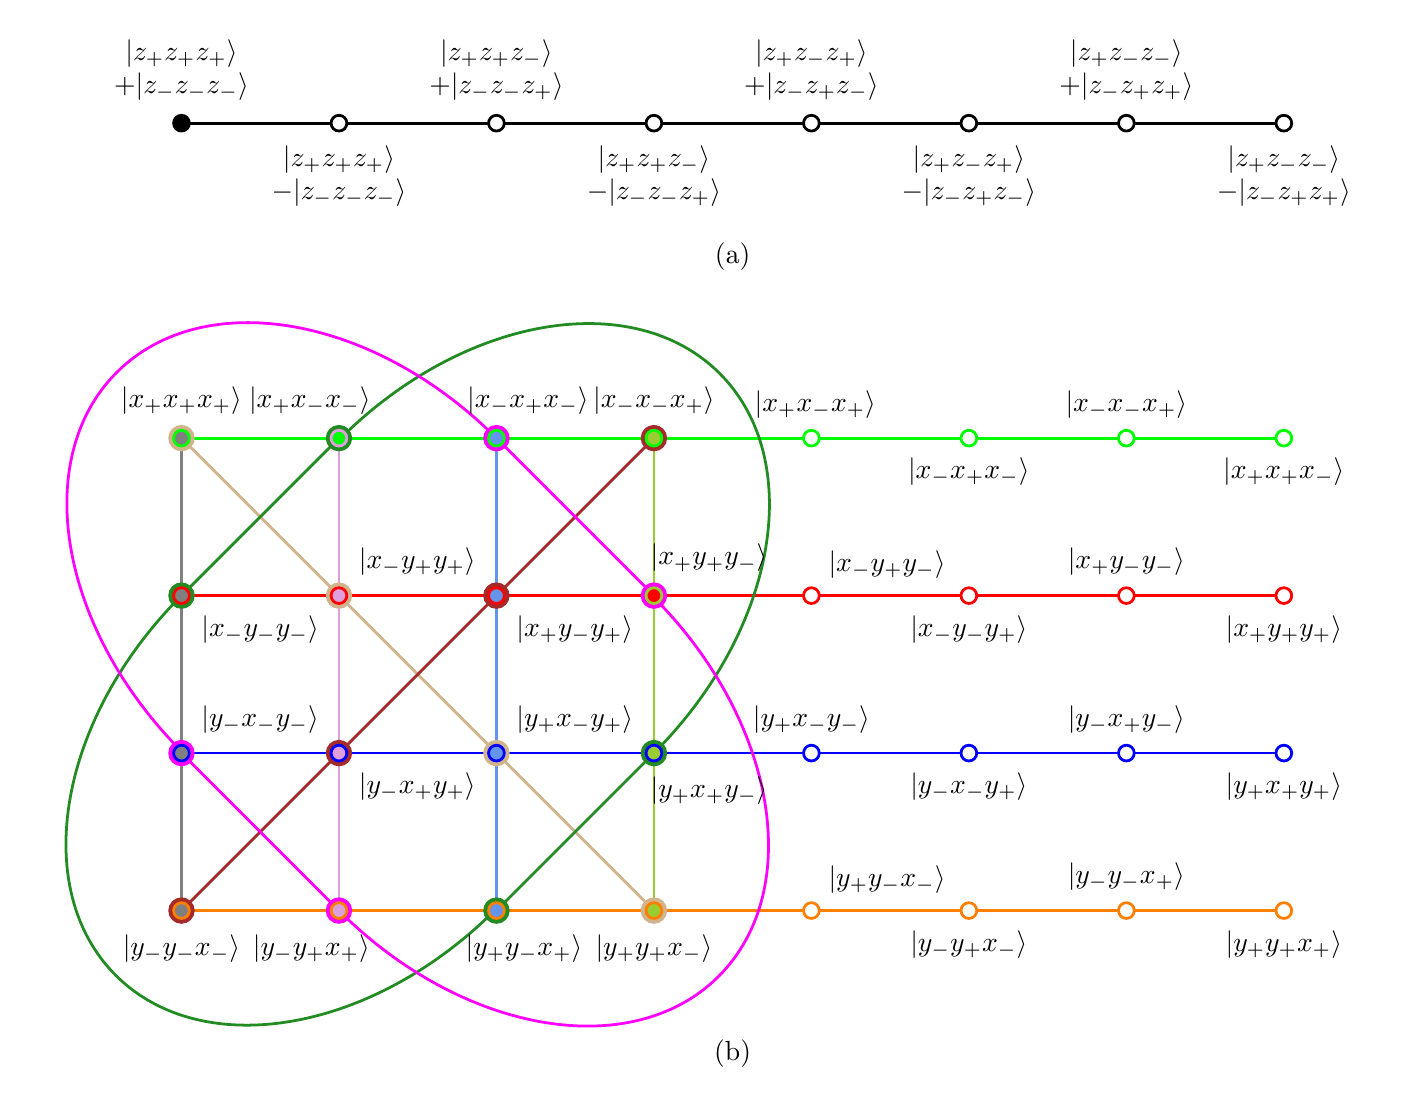
\begin{tikzpicture}  [scale=1]

\tikzstyle{every path}=[line width=1pt]

\newdimen\ms
\ms=0.1cm
\tikzstyle{s1}=[color=red,rectangle,inner sep=3.5]
\tikzstyle{c3}=[circle,inner sep={\ms/8},minimum size=4*\ms]
\tikzstyle{c2}=[circle,inner sep={\ms/8},minimum size=3*\ms]
\tikzstyle{c1}=[circle,inner sep={\ms/8},minimum size=2*\ms]
\tikzstyle{cs1}=[circle,inner sep={\ms/8},minimum size=1*\ms]

% Define positions of all observables

\coordinate (uuu) at (0,10);
\coordinate (uuv) at (2,10);
\coordinate (uvu) at (4,10);
\coordinate (uvv) at (6,10);
\coordinate (vuu) at (8,10);
\coordinate (vuv) at (10,10);
\coordinate (vvu) at (12,10);
\coordinate (vvv) at (14,10);

% draw contexts

\draw [color=black] (uuu) -- (vvv);

% draw atoms

\draw (uuu) coordinate[c1,fill=black, draw=black,label=above:{\begin{tabular}{c} $\vert z_+z_+z_+ \rangle $\\$ + \vert z_-z_-z_- \rangle $\end{tabular}}];
\draw (uuv) coordinate[c1,fill=white, draw=black,label=below:{\begin{tabular}{c} $\vert z_+z_+z_+ \rangle $\\$ - \vert z_-z_-z_- \rangle $\end{tabular}}];
\draw (uvu) coordinate[c1,fill=white, draw=black,label=above:{\begin{tabular}{c} $\vert z_+z_+z_- \rangle $\\$ + \vert z_-z_-z_+ \rangle $\end{tabular}}];
\draw (uvv) coordinate[c1,fill=white, draw=black,label=below:{\begin{tabular}{c} $\vert z_+z_+z_- \rangle $\\$ - \vert z_-z_-z_+ \rangle $\end{tabular}}];
\draw (vuu) coordinate[c1,fill=white, draw=black,label=above:{\begin{tabular}{c} $\vert z_+z_-z_+ \rangle $\\$ + \vert z_-z_+z_- \rangle $\end{tabular}}];
\draw (vuv) coordinate[c1,fill=white, draw=black,label=below:{\begin{tabular}{c} $\vert z_+z_-z_+ \rangle $\\$ - \vert z_-z_+z_- \rangle $\end{tabular}}];
\draw (vvu) coordinate[c1,fill=white, draw=black,label=above:{\begin{tabular}{c} $\vert z_+z_-z_- \rangle $\\$ + \vert z_-z_+z_+ \rangle $\end{tabular}}];
\draw (vvv) coordinate[c1,fill=white, draw=black,label=below:{\begin{tabular}{c} $\vert z_+z_-z_- \rangle $\\$ - \vert z_-z_+z_+ \rangle $\end{tabular}}];

\coordinate (a) at (7,8);
\draw (a) coordinate[label=above:(a)];

% Define positions of all observables

\coordinate (uuu) at ( 0,6);
\coordinate (uuv) at ( 2,6);
\coordinate (uvu) at ( 4,6);
\coordinate (uvv) at ( 6,6);
\coordinate (vuu) at ( 8,6);
\coordinate (vuv) at (10,6);
\coordinate (vvu) at (12,6);
\coordinate (vvv) at (14,6);


\coordinate (ucc) at ( 0,4);
\coordinate (vcc) at ( 2,4);
\coordinate (ucd) at ( 4,4);
\coordinate (vcd) at ( 6,4);
\coordinate (udc) at ( 8,4);
\coordinate (vdc) at (10,4);
\coordinate (udd) at (12,4);
\coordinate (vdd) at (14,4);

\coordinate (cuc) at ( 0,2);
\coordinate (cvc) at ( 2,2);
\coordinate (cud) at ( 4,2);
\coordinate (cvd) at ( 6,2);
\coordinate (duc) at ( 8,2);
\coordinate (dvc) at (10,2);
\coordinate (dud) at (12,2);
\coordinate (dvd) at (14,2);

\coordinate (ccu) at ( 0,0);
\coordinate (ccv) at ( 2,0);
\coordinate (cdu) at ( 4,0);
\coordinate (cdv) at ( 6,0);
\coordinate (dcu) at ( 8,0);
\coordinate (dcv) at (10,0);
\coordinate (ddu) at (12,0);
\coordinate (ddv) at (14,0);




% draw contexts

\draw [color=orange] (ccu) -- (ddv);
\draw [color=blue] (cuc) -- (dvd);
\draw [color=red] (ucc) -- (vdd);
\draw [color=green] (uuu) -- (vvv);

\draw [color=Gray] (uuu) -- (ccu);
\draw [color=Plum] (uuv) -- (ccv);
\draw [color=CornflowerBlue] (uvu) -- (cdu);
\draw [color=YellowGreen] (uvv) -- (cdv);


\draw [color=Tan] (uuu) -- (cdv);
\draw [color=Brown] (uvv) -- (ccu);


\draw [color=ForestGreen] (uuv) -- (ucc);
\draw [color=ForestGreen](cdu) -- (cvd);
\draw [rotate=225,color=ForestGreen] (cvd) arc (90:270:4 and 2.82);
\draw[rotate=45,color=ForestGreen] (ucc) arc (90:270:4 and 2.82);

\draw [color=Magenta] (cuc) -- (ccv);
\draw [color=Magenta] (uvu) -- (vcd);
\draw[rotate=315,color=Magenta] (uvu) arc (90:270:4 and 2.82);
\draw[rotate=135,color=Magenta] (ccv) arc (90:270:4 and 2.82);


% draw atoms


 \draw (uuu) coordinate[c2,fill=Tan, draw=Tan,label=above:$\vert x_+  x_+  x_+  \rangle $];
 \draw (uuu) coordinate[c1,fill=Gray, draw=green];
 \draw (uuv) coordinate[c2,fill=ForestGreen, draw=ForestGreen,label={[xshift=-3.7mm]90:$\vert x_+  x_-  x_-  \rangle $}];
 \draw (uuv) coordinate[c1,fill=green, draw=Plum];
 \draw (uvu) coordinate[c2,fill=Magenta, draw=Magenta,label={[xshift=+4mm]90:$\vert x_-  x_+  x_-  \rangle $}];
 \draw (uvu) coordinate[c1,fill=CornflowerBlue, draw=green];
 \draw (uvv) coordinate[c2,fill=Brown, draw=Brown,label=above:$\vert x_-  x_-  x_+  \rangle $];
 \draw (uvv) coordinate[c1,fill=YellowGreen, draw=green];
 \draw (vuu) coordinate[c1,fill=white, draw=green,label={[xshift=+0.5mm]90:$\vert x_+x_-x_+      \rangle $}];
 \draw (vuv) coordinate[c1,fill=white, draw=green,label=below:$\vert x_-x_+x_-      \rangle $];
 \draw (vvu) coordinate[c1,fill=white, draw=green,label=above:$\vert x_-x_-x_+      \rangle $];
 \draw (vvv) coordinate[c1,fill=white, draw=green,label=below:$\vert x_+x_+x_-      \rangle $];


  % \draw (ucc) coordinate[c2,fill=ForestGreen, draw=ForestGreen,label={[xshift=-7.5mm,distance=0mm]90:$\vert x_-  y_-  y_-  \rangle $}];
   \draw (ucc) coordinate[c2,fill=ForestGreen, draw=ForestGreen,label=below right:$\vert x_-  y_-  y_-  \rangle $];
   \draw (ucc) coordinate[c1,fill=Gray, draw=red];
   \draw (vcc) coordinate[c2,fill=Tan, draw=Tan,label=above right:$\vert x_-  y_+  y_+  \rangle $];
   \draw (vcc) coordinate[c1,fill=Plum, draw=red];
   \draw (ucd) coordinate[c2,fill=Brown, draw=Brown,label=below right:$\vert x_+  y_-  y_+  \rangle $];
   \draw (ucd) coordinate[c1,fill=CornflowerBlue, draw=red];
  % \draw (vcd) coordinate[c2,fill=Magenta, draw=Magenta,label=above right:$\vert x_+  y_+  y_-  \rangle $];
   \draw (vcd) coordinate[c2,fill=Magenta, draw=Magenta,label={[xshift=+7mm,distance=12mm]90:$\vert x_+  y_+  y_-  \rangle $}];
   \draw (vcd) coordinate[c1,fill=red, draw=YellowGreen];
   \draw (udc) coordinate[c1,fill=white, draw=red,label=above right:$\vert x_-y_+y_-      \rangle $];
   \draw (vdc) coordinate[c1,fill=white, draw=red,label=below:$\vert x_-y_-y_+      \rangle $];
   \draw (udd) coordinate[c1,fill=white, draw=red,label=above:$\vert x_+y_-y_-      \rangle $];
   \draw (vdd) coordinate[c1,fill=white, draw=red,label=below:$\vert x_+y_+y_+      \rangle $];

  \draw (cuc) coordinate[c2,fill=Magenta, draw=Magenta,label=above right:$\vert y_-  x_-  y_-  \rangle $];
  \draw (cuc) coordinate[c1,fill=Gray, draw=blue];
  \draw (cvc) coordinate[c2,fill=Brown, draw=Brown,label=below right:$\vert y_-  x_+  y_+  \rangle $];
  \draw (cvc) coordinate[c1,fill=Plum, draw=blue];
  \draw (cud) coordinate[c2,fill=Tan, draw=Tan,label=above right:$\vert y_+  x_-  y_+  \rangle $];
  \draw (cud) coordinate[c1,fill=CornflowerBlue, draw=blue];
  \draw (cvd) coordinate[c2,fill=ForestGreen, draw=ForestGreen,label={[xshift=+7mm,distance=12mm]270:$\vert y_+  x_+  y_-  \rangle $}];
  \draw (cvd) coordinate[c1,fill=YellowGreen, draw=blue];
  \draw (duc) coordinate[c1,fill=white, draw=blue,label=above:$\vert y_+x_-y_-      \rangle $];
  \draw (dvc) coordinate[c1,fill=white, draw=blue,label=below:$\vert y_-x_-y_+      \rangle $];
  \draw (dud) coordinate[c1,fill=white, draw=blue,label=above:$\vert y_-x_+y_-      \rangle $];
  \draw (dvd) coordinate[c1,fill=white, draw=blue,label=below:$\vert y_+x_+y_+      \rangle $];

\draw (ccu) coordinate[c2,fill=Brown, draw=Brown,label=below:$\vert y_-  y_-  x_-  \rangle $];
\draw (ccu) coordinate[c1,fill=Gray, draw=orange];
\draw (ccv) coordinate[c2,fill=Magenta, draw=Magenta,label={[xshift=-3.5mm]270:$\vert y_-  y_+  x_+  \rangle $}];
\draw (ccv) coordinate[c1,fill=Plum, draw=orange];
\draw (cdu) coordinate[c2,fill=ForestGreen, draw=ForestGreen,label={[xshift=+3.5mm]270:$\vert y_+  y_-  x_+  \rangle $}];
\draw (cdu) coordinate[c1,fill=CornflowerBlue, draw=orange];
\draw (cdv) coordinate[c2,fill=Tan, draw=Tan,label=below:$\vert y_+  y_+  x_-  \rangle $];
\draw (cdv) coordinate[c1,fill=YellowGreen, draw=orange];
\draw (dcu) coordinate[c1,fill=white, draw=orange,label=above right:$\vert y_+y_-x_-      \rangle $];
\draw (dcv) coordinate[c1,fill=white, draw=orange,label=below:$\vert y_-y_+x_-      \rangle $];
\draw (ddu) coordinate[c1,fill=white, draw=orange,label=above:$\vert y_-y_-x_+      \rangle $];
\draw (ddv) coordinate[c1,fill=white, draw=orange,label=below:$\vert y_+y_+x_+      \rangle $];


\coordinate (b) at (7,-1.5);
\draw (b) coordinate[label=below:(b)];

\end{tikzpicture}
\end{center}
\caption{\label{2020-f-ghz-contextqm}
Hypergraphs representing  (a) the single quantum mechanical GHZ context in the GHZ basiswhich are the eigenstates of $\sigma_z \sigma_z \sigma_z$,
and (b) the 12 tightly intertwined GHZ contexts in the bases of the eigenstates of
$\sigma_y \sigma_y \sigma_x$, $\sigma_y \sigma_x \sigma_y$, $\sigma_x \sigma_y \sigma_y$,  and $\sigma_x \sigma_x \sigma_x$
with 8 atoms each.
Filled circles indicate states allowed by the original GHZ game yielding a discord with classical means and predictions.
}
\end{figure*}

\section{Classical contextuality or context dependence}

An examination of the subgraph of the GHZ logic hypergraph, depicted in Figure~\ref{2020-f-ghz-contextqm}(b) ``covered'' by $\vert \Upsilon_1 \rangle$
shows that this (sub)logic has a separating set of eight admissible two-valued states
satisfying completeness (every context contains a red or 1 value) and exclusivity (every context contains only one red or 1 value, all other vertices are green or 0 value)
drawn in Figure~\ref{2020-f-ghz-contextghz2vs}. (In this presentation the two-valued states appear like permutation matrices.)
Therefore this GHZ (sub)logic has a classical
representation by a partition logic $\{1,2,\ldots ,8\}$ of eight elements, as drawn in Figure~\ref{2020-f-ghz-contextpl}.

\begin{figure}[htb!]%[H]
\begin{center}
\begin{tabular}{ c c }
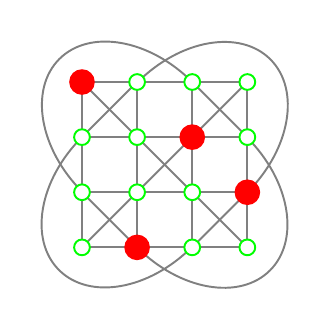
\begin{tikzpicture}  [scale=0.35]

\tikzstyle{every path}=[line width=0.7pt]

\newdimen\ms
\ms=0.1cm
\tikzstyle{s1}=[color=red,rectangle,inner sep=3.5]
\tikzstyle{c3}=[circle,inner sep={\ms/8},minimum size=4*\ms]
\tikzstyle{c2}=[circle,inner sep={\ms/8},minimum size=3*\ms]
\tikzstyle{c1}=[circle,inner sep={\ms/8},minimum size=2*\ms]
\tikzstyle{cs1}=[circle,inner sep={\ms/8},minimum size=1*\ms]

% Define positions of all observables

\coordinate (uuu) at ( 0,6);
\coordinate (uuv) at ( 2,6);
\coordinate (uvu) at ( 4,6);
\coordinate (uvv) at ( 6,6);
\coordinate (vuu) at ( 8,6);
\coordinate (vuv) at (10,6);
\coordinate (vvu) at (12,6);
\coordinate (vvv) at (14,6);

\coordinate (ucc) at ( 0,4);
\coordinate (vcc) at ( 2,4);
\coordinate (ucd) at ( 4,4);
\coordinate (vcd) at ( 6,4);
\coordinate (udc) at ( 8,4);
\coordinate (vdc) at (10,4);
\coordinate (udd) at (12,4);
\coordinate (vdd) at (14,4);

\coordinate (cuc) at ( 0,2);
\coordinate (cvc) at ( 2,2);
\coordinate (cud) at ( 4,2);
\coordinate (cvd) at ( 6,2);
\coordinate (duc) at ( 8,2);
\coordinate (dvc) at (10,2);
\coordinate (dud) at (12,2);
\coordinate (dvd) at (14,2);

\coordinate (ccu) at ( 0,0);
\coordinate (ccv) at ( 2,0);
\coordinate (cdu) at ( 4,0);
\coordinate (cdv) at ( 6,0);
\coordinate (dcu) at ( 8,0);
\coordinate (dcv) at (10,0);
\coordinate (ddu) at (12,0);
\coordinate (ddv) at (14,0);

% draw contexts

\draw [color=Gray] (ccu) -- (cdv);
\draw [color=Gray] (cuc) -- (cvd);
\draw [color=Gray] (ucc) -- (vcd);
\draw [color=Gray] (uuu) -- (uvv);

\draw [color=Gray] (uuu) -- (ccu);
\draw [color=Gray] (uuv) -- (ccv);
\draw [color=Gray] (uvu) -- (cdu);
\draw [color=Gray] (uvv) -- (cdv);

\draw [color=Gray] (uuu) -- (cdv);
\draw [color=Gray] (uvv) -- (ccu);

\draw [color=Gray] (uuv) -- (ucc);
\draw [color=Gray](cdu) -- (cvd);
\draw [rotate=225,color=Gray] (cvd) arc (90:270:4 and 2.82);
\draw[rotate=45,color=Gray] (ucc) arc (90:270:4 and 2.82);

\draw [color=Gray] (cuc) -- (ccv);
\draw [color=Gray] (uvu) -- (vcd);
\draw[rotate=315,color=Gray] (uvu) arc (90:270:4 and 2.82);
\draw[rotate=135,color=Gray] (ccv) arc (90:270:4 and 2.82);

%draw atoms

\draw (uuu) coordinate[c2,fill=red,draw=red];
\draw (uuv) coordinate[c1,fill=white,draw=green];
\draw (uvu) coordinate[c1,fill=white,draw=green];
\draw (uvv) coordinate[c1,fill=white,draw=green];


\draw (ucc) coordinate[c1,fill=white,draw=green];
\draw (vcc) coordinate[c1,fill=white,draw=green];
\draw (ucd) coordinate[c2,fill=red,draw=red];
\draw (vcd) coordinate[c1,fill=white,draw=green];

\draw (cuc) coordinate[c1,fill=white,draw=green];
\draw (cvc) coordinate[c1,fill=white,draw=green];
\draw (cud) coordinate[c1,fill=white,draw=green];
\draw (cvd) coordinate[c2,fill=red,draw=red];

\draw (ccu) coordinate[c1,fill=white,draw=green];
\draw (ccv) coordinate[c2,fill=red,draw=red];
\draw (cdu) coordinate[c1,fill=white,draw=green];
\draw (cdv) coordinate[c1,fill=white,draw=green];

\end{tikzpicture}
%%%%%%%%%%%%% 2
&
%
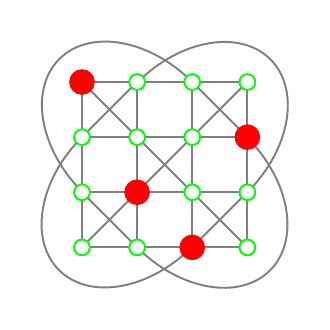
\begin{tikzpicture}  [scale=0.35]

\tikzstyle{every path}=[line width=0.7pt]

\newdimen\ms
\ms=0.1cm
\tikzstyle{s1}=[color=red,rectangle,inner sep=3.5]
\tikzstyle{c3}=[circle,inner sep={\ms/8},minimum size=4*\ms]
\tikzstyle{c2}=[circle,inner sep={\ms/8},minimum size=3*\ms]
\tikzstyle{c1}=[circle,inner sep={\ms/8},minimum size=2*\ms]
\tikzstyle{cs1}=[circle,inner sep={\ms/8},minimum size=1*\ms]

% Define positions of all observables

\coordinate (uuu) at ( 0,6);
\coordinate (uuv) at ( 2,6);
\coordinate (uvu) at ( 4,6);
\coordinate (uvv) at ( 6,6);
\coordinate (vuu) at ( 8,6);
\coordinate (vuv) at (10,6);
\coordinate (vvu) at (12,6);
\coordinate (vvv) at (14,6);

\coordinate (ucc) at ( 0,4);
\coordinate (vcc) at ( 2,4);
\coordinate (ucd) at ( 4,4);
\coordinate (vcd) at ( 6,4);
\coordinate (udc) at ( 8,4);
\coordinate (vdc) at (10,4);
\coordinate (udd) at (12,4);
\coordinate (vdd) at (14,4);

\coordinate (cuc) at ( 0,2);
\coordinate (cvc) at ( 2,2);
\coordinate (cud) at ( 4,2);
\coordinate (cvd) at ( 6,2);
\coordinate (duc) at ( 8,2);
\coordinate (dvc) at (10,2);
\coordinate (dud) at (12,2);
\coordinate (dvd) at (14,2);

\coordinate (ccu) at ( 0,0);
\coordinate (ccv) at ( 2,0);
\coordinate (cdu) at ( 4,0);
\coordinate (cdv) at ( 6,0);
\coordinate (dcu) at ( 8,0);
\coordinate (dcv) at (10,0);
\coordinate (ddu) at (12,0);
\coordinate (ddv) at (14,0);

% draw contexts

\draw [color=Gray] (ccu) -- (cdv);
\draw [color=Gray] (cuc) -- (cvd);
\draw [color=Gray] (ucc) -- (vcd);
\draw [color=Gray] (uuu) -- (uvv);

\draw [color=Gray] (uuu) -- (ccu);
\draw [color=Gray] (uuv) -- (ccv);
\draw [color=Gray] (uvu) -- (cdu);
\draw [color=Gray] (uvv) -- (cdv);

\draw [color=Gray] (uuu) -- (cdv);
\draw [color=Gray] (uvv) -- (ccu);

\draw [color=Gray] (uuv) -- (ucc);
\draw [color=Gray](cdu) -- (cvd);
\draw [rotate=225,color=Gray] (cvd) arc (90:270:4 and 2.82);
\draw[rotate=45,color=Gray] (ucc) arc (90:270:4 and 2.82);

\draw [color=Gray] (cuc) -- (ccv);
\draw [color=Gray] (uvu) -- (vcd);
\draw[rotate=315,color=Gray] (uvu) arc (90:270:4 and 2.82);
\draw[rotate=135,color=Gray] (ccv) arc (90:270:4 and 2.82);

%draw atoms

\draw (uuu) coordinate[c2,fill=red,draw=red];
\draw (uuv) coordinate[c1,fill=white,draw=green];
\draw (uvu) coordinate[c1,fill=white,draw=green];
\draw (uvv) coordinate[c1,fill=white,draw=green];


\draw (ucc) coordinate[c1,fill=white,draw=green];
\draw (vcc) coordinate[c1,fill=white,draw=green];
\draw (ucd) coordinate[c1,fill=white,draw=green];
\draw (vcd) coordinate[c2,fill=red,draw=red];

\draw (cuc) coordinate[c1,fill=white,draw=green];
\draw (cvc) coordinate[c2,fill=red,draw=red];
\draw (cud) coordinate[c1,fill=white,draw=green];
\draw (cvd) coordinate[c1,fill=white,draw=green];

\draw (ccu) coordinate[c1,fill=white,draw=green];
\draw (ccv) coordinate[c1,fill=white,draw=green];
\draw (cdu) coordinate[c2,fill=red,draw=red];
\draw (cdv) coordinate[c1,fill=white,draw=green];

\end{tikzpicture}
%
\\
%%%%%%%%%%%%%% 3
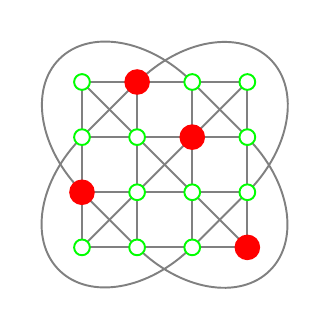
\begin{tikzpicture}  [scale=0.35]

\tikzstyle{every path}=[line width=0.7pt]

\newdimen\ms
\ms=0.1cm
\tikzstyle{s1}=[color=red,rectangle,inner sep=3.5]
\tikzstyle{c3}=[circle,inner sep={\ms/8},minimum size=4*\ms]
\tikzstyle{c2}=[circle,inner sep={\ms/8},minimum size=3*\ms]
\tikzstyle{c1}=[circle,inner sep={\ms/8},minimum size=2*\ms]
\tikzstyle{cs1}=[circle,inner sep={\ms/8},minimum size=1*\ms]

% Define positions of all observables

\coordinate (uuu) at ( 0,6);
\coordinate (uuv) at ( 2,6);
\coordinate (uvu) at ( 4,6);
\coordinate (uvv) at ( 6,6);
\coordinate (vuu) at ( 8,6);
\coordinate (vuv) at (10,6);
\coordinate (vvu) at (12,6);
\coordinate (vvv) at (14,6);

\coordinate (ucc) at ( 0,4);
\coordinate (vcc) at ( 2,4);
\coordinate (ucd) at ( 4,4);
\coordinate (vcd) at ( 6,4);
\coordinate (udc) at ( 8,4);
\coordinate (vdc) at (10,4);
\coordinate (udd) at (12,4);
\coordinate (vdd) at (14,4);

\coordinate (cuc) at ( 0,2);
\coordinate (cvc) at ( 2,2);
\coordinate (cud) at ( 4,2);
\coordinate (cvd) at ( 6,2);
\coordinate (duc) at ( 8,2);
\coordinate (dvc) at (10,2);
\coordinate (dud) at (12,2);
\coordinate (dvd) at (14,2);

\coordinate (ccu) at ( 0,0);
\coordinate (ccv) at ( 2,0);
\coordinate (cdu) at ( 4,0);
\coordinate (cdv) at ( 6,0);
\coordinate (dcu) at ( 8,0);
\coordinate (dcv) at (10,0);
\coordinate (ddu) at (12,0);
\coordinate (ddv) at (14,0);

% draw contexts

\draw [color=Gray] (ccu) -- (cdv);
\draw [color=Gray] (cuc) -- (cvd);
\draw [color=Gray] (ucc) -- (vcd);
\draw [color=Gray] (uuu) -- (uvv);

\draw [color=Gray] (uuu) -- (ccu);
\draw [color=Gray] (uuv) -- (ccv);
\draw [color=Gray] (uvu) -- (cdu);
\draw [color=Gray] (uvv) -- (cdv);

\draw [color=Gray] (uuu) -- (cdv);
\draw [color=Gray] (uvv) -- (ccu);

\draw [color=Gray] (uuv) -- (ucc);
\draw [color=Gray](cdu) -- (cvd);
\draw [rotate=225,color=Gray] (cvd) arc (90:270:4 and 2.82);
\draw[rotate=45,color=Gray] (ucc) arc (90:270:4 and 2.82);

\draw [color=Gray] (cuc) -- (ccv);
\draw [color=Gray] (uvu) -- (vcd);
\draw[rotate=315,color=Gray] (uvu) arc (90:270:4 and 2.82);
\draw[rotate=135,color=Gray] (ccv) arc (90:270:4 and 2.82);

%draw atoms

\draw (uuu) coordinate[c1,fill=white,draw=green];
\draw (uuv) coordinate[c2,fill=red,draw=red];
\draw (uvu) coordinate[c1,fill=white,draw=green];
\draw (uvv) coordinate[c1,fill=white,draw=green];


\draw (ucc) coordinate[c1,fill=white,draw=green];
\draw (vcc) coordinate[c1,fill=white,draw=green];
\draw (ucd) coordinate[c2,fill=red,draw=red];
\draw (vcd) coordinate[c1,fill=white,draw=green];

\draw (cuc) coordinate[c2,fill=red,draw=red];
\draw (cvc) coordinate[c1,fill=white,draw=green];
\draw (cud) coordinate[c1,fill=white,draw=green];
\draw (cvd) coordinate[c1,fill=white,draw=green];

\draw (ccu) coordinate[c1,fill=white,draw=green];
\draw (ccv) coordinate[c1,fill=white,draw=green];
\draw (cdu) coordinate[c1,fill=white,draw=green];
\draw (cdv) coordinate[c2,fill=red,draw=red];

\end{tikzpicture}
%
&
%
%%%%%%%%%% 4
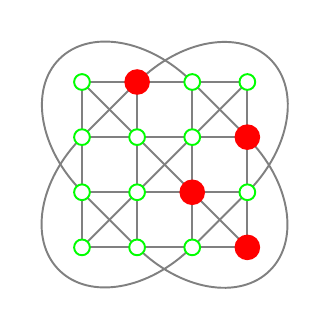
\begin{tikzpicture}  [scale=0.35]

\tikzstyle{every path}=[line width=0.7pt]

\newdimen\ms
\ms=0.1cm
\tikzstyle{s1}=[color=red,rectangle,inner sep=3.5]
\tikzstyle{c3}=[circle,inner sep={\ms/8},minimum size=4*\ms]
\tikzstyle{c2}=[circle,inner sep={\ms/8},minimum size=3*\ms]
\tikzstyle{c1}=[circle,inner sep={\ms/8},minimum size=2*\ms]
\tikzstyle{cs1}=[circle,inner sep={\ms/8},minimum size=1*\ms]

% Define positions of all observables

\coordinate (uuu) at ( 0,6);
\coordinate (uuv) at ( 2,6);
\coordinate (uvu) at ( 4,6);
\coordinate (uvv) at ( 6,6);
\coordinate (vuu) at ( 8,6);
\coordinate (vuv) at (10,6);
\coordinate (vvu) at (12,6);
\coordinate (vvv) at (14,6);

\coordinate (ucc) at ( 0,4);
\coordinate (vcc) at ( 2,4);
\coordinate (ucd) at ( 4,4);
\coordinate (vcd) at ( 6,4);
\coordinate (udc) at ( 8,4);
\coordinate (vdc) at (10,4);
\coordinate (udd) at (12,4);
\coordinate (vdd) at (14,4);

\coordinate (cuc) at ( 0,2);
\coordinate (cvc) at ( 2,2);
\coordinate (cud) at ( 4,2);
\coordinate (cvd) at ( 6,2);
\coordinate (duc) at ( 8,2);
\coordinate (dvc) at (10,2);
\coordinate (dud) at (12,2);
\coordinate (dvd) at (14,2);

\coordinate (ccu) at ( 0,0);
\coordinate (ccv) at ( 2,0);
\coordinate (cdu) at ( 4,0);
\coordinate (cdv) at ( 6,0);
\coordinate (dcu) at ( 8,0);
\coordinate (dcv) at (10,0);
\coordinate (ddu) at (12,0);
\coordinate (ddv) at (14,0);

% draw contexts

\draw [color=Gray] (ccu) -- (cdv);
\draw [color=Gray] (cuc) -- (cvd);
\draw [color=Gray] (ucc) -- (vcd);
\draw [color=Gray] (uuu) -- (uvv);

\draw [color=Gray] (uuu) -- (ccu);
\draw [color=Gray] (uuv) -- (ccv);
\draw [color=Gray] (uvu) -- (cdu);
\draw [color=Gray] (uvv) -- (cdv);

\draw [color=Gray] (uuu) -- (cdv);
\draw [color=Gray] (uvv) -- (ccu);

\draw [color=Gray] (uuv) -- (ucc);
\draw [color=Gray](cdu) -- (cvd);
\draw [rotate=225,color=Gray] (cvd) arc (90:270:4 and 2.82);
\draw[rotate=45,color=Gray] (ucc) arc (90:270:4 and 2.82);

\draw [color=Gray] (cuc) -- (ccv);
\draw [color=Gray] (uvu) -- (vcd);
\draw[rotate=315,color=Gray] (uvu) arc (90:270:4 and 2.82);
\draw[rotate=135,color=Gray] (ccv) arc (90:270:4 and 2.82);

%draw atoms

\draw (uuu) coordinate[c1,fill=white,draw=green];
\draw (uuv) coordinate[c2,fill=red,draw=red];
\draw (uvu) coordinate[c1,fill=white,draw=green];
\draw (uvv) coordinate[c1,fill=white,draw=green];


\draw (ucc) coordinate[c1,fill=white,draw=green];
\draw (vcc) coordinate[c1,fill=white,draw=green];
\draw (ucd) coordinate[c1,fill=white,draw=green];
\draw (vcd) coordinate[c2,fill=red,draw=red];

\draw (cuc) coordinate[c1,fill=white,draw=green];
\draw (cvc) coordinate[c1,fill=white,draw=green];
\draw (cud) coordinate[c2,fill=red,draw=red];
\draw (cvd) coordinate[c1,fill=white,draw=green];

\draw (ccu) coordinate[c1,fill=white,draw=green];
\draw (ccv) coordinate[c1,fill=white,draw=green];
\draw (cdu) coordinate[c1,fill=white,draw=green];
\draw (cdv) coordinate[c2,fill=red,draw=red];

\end{tikzpicture}
%
%
\\
%
%%%%%%%%%%% 5
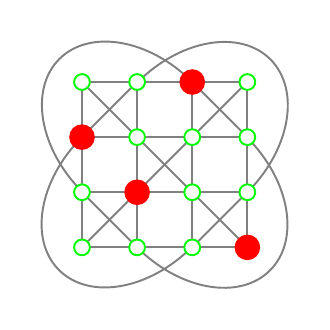
\begin{tikzpicture}  [scale=0.35]

\tikzstyle{every path}=[line width=0.7pt]

\newdimen\ms
\ms=0.1cm
\tikzstyle{s1}=[color=red,rectangle,inner sep=3.5]
\tikzstyle{c3}=[circle,inner sep={\ms/8},minimum size=4*\ms]
\tikzstyle{c2}=[circle,inner sep={\ms/8},minimum size=3*\ms]
\tikzstyle{c1}=[circle,inner sep={\ms/8},minimum size=2*\ms]
\tikzstyle{cs1}=[circle,inner sep={\ms/8},minimum size=1*\ms]

% Define positions of all observables

\coordinate (uuu) at ( 0,6);
\coordinate (uuv) at ( 2,6);
\coordinate (uvu) at ( 4,6);
\coordinate (uvv) at ( 6,6);
\coordinate (vuu) at ( 8,6);
\coordinate (vuv) at (10,6);
\coordinate (vvu) at (12,6);
\coordinate (vvv) at (14,6);

\coordinate (ucc) at ( 0,4);
\coordinate (vcc) at ( 2,4);
\coordinate (ucd) at ( 4,4);
\coordinate (vcd) at ( 6,4);
\coordinate (udc) at ( 8,4);
\coordinate (vdc) at (10,4);
\coordinate (udd) at (12,4);
\coordinate (vdd) at (14,4);

\coordinate (cuc) at ( 0,2);
\coordinate (cvc) at ( 2,2);
\coordinate (cud) at ( 4,2);
\coordinate (cvd) at ( 6,2);
\coordinate (duc) at ( 8,2);
\coordinate (dvc) at (10,2);
\coordinate (dud) at (12,2);
\coordinate (dvd) at (14,2);

\coordinate (ccu) at ( 0,0);
\coordinate (ccv) at ( 2,0);
\coordinate (cdu) at ( 4,0);
\coordinate (cdv) at ( 6,0);
\coordinate (dcu) at ( 8,0);
\coordinate (dcv) at (10,0);
\coordinate (ddu) at (12,0);
\coordinate (ddv) at (14,0);

% draw contexts

\draw [color=Gray] (ccu) -- (cdv);
\draw [color=Gray] (cuc) -- (cvd);
\draw [color=Gray] (ucc) -- (vcd);
\draw [color=Gray] (uuu) -- (uvv);

\draw [color=Gray] (uuu) -- (ccu);
\draw [color=Gray] (uuv) -- (ccv);
\draw [color=Gray] (uvu) -- (cdu);
\draw [color=Gray] (uvv) -- (cdv);

\draw [color=Gray] (uuu) -- (cdv);
\draw [color=Gray] (uvv) -- (ccu);

\draw [color=Gray] (uuv) -- (ucc);
\draw [color=Gray](cdu) -- (cvd);
\draw [rotate=225,color=Gray] (cvd) arc (90:270:4 and 2.82);
\draw[rotate=45,color=Gray] (ucc) arc (90:270:4 and 2.82);

\draw [color=Gray] (cuc) -- (ccv);
\draw [color=Gray] (uvu) -- (vcd);
\draw[rotate=315,color=Gray] (uvu) arc (90:270:4 and 2.82);
\draw[rotate=135,color=Gray] (ccv) arc (90:270:4 and 2.82);

%draw atoms

\draw (uuu) coordinate[c1,fill=white,draw=green];
\draw (uuv) coordinate[c1,fill=white,draw=green];
\draw (uvu) coordinate[c2,fill=red,draw=red];
\draw (uvv) coordinate[c1,fill=white,draw=green];


\draw (ucc) coordinate[c2,fill=red,draw=red];
\draw (vcc) coordinate[c1,fill=white,draw=green];
\draw (ucd) coordinate[c1,fill=white,draw=green];
\draw (vcd) coordinate[c1,fill=white,draw=green];

\draw (cuc) coordinate[c1,fill=white,draw=green];
\draw (cvc) coordinate[c2,fill=red,draw=red];
\draw (cud) coordinate[c1,fill=white,draw=green];
\draw (cvd) coordinate[c1,fill=white,draw=green];

\draw (ccu) coordinate[c1,fill=white,draw=green];
\draw (ccv) coordinate[c1,fill=white,draw=green];
\draw (cdu) coordinate[c1,fill=white,draw=green];
\draw (cdv) coordinate[c2,fill=red,draw=red];

\end{tikzpicture}
%
&
%
%%%%%%%%%%%%%%%%%%% 6
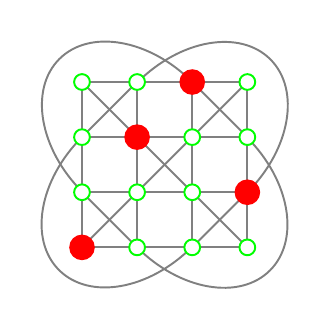
\begin{tikzpicture}  [scale=0.35]

\tikzstyle{every path}=[line width=0.7pt]

\newdimen\ms
\ms=0.1cm
\tikzstyle{s1}=[color=red,rectangle,inner sep=3.5]
\tikzstyle{c3}=[circle,inner sep={\ms/8},minimum size=4*\ms]
\tikzstyle{c2}=[circle,inner sep={\ms/8},minimum size=3*\ms]
\tikzstyle{c1}=[circle,inner sep={\ms/8},minimum size=2*\ms]
\tikzstyle{cs1}=[circle,inner sep={\ms/8},minimum size=1*\ms]

% Define positions of all observables

\coordinate (uuu) at ( 0,6);
\coordinate (uuv) at ( 2,6);
\coordinate (uvu) at ( 4,6);
\coordinate (uvv) at ( 6,6);
\coordinate (vuu) at ( 8,6);
\coordinate (vuv) at (10,6);
\coordinate (vvu) at (12,6);
\coordinate (vvv) at (14,6);

\coordinate (ucc) at ( 0,4);
\coordinate (vcc) at ( 2,4);
\coordinate (ucd) at ( 4,4);
\coordinate (vcd) at ( 6,4);
\coordinate (udc) at ( 8,4);
\coordinate (vdc) at (10,4);
\coordinate (udd) at (12,4);
\coordinate (vdd) at (14,4);

\coordinate (cuc) at ( 0,2);
\coordinate (cvc) at ( 2,2);
\coordinate (cud) at ( 4,2);
\coordinate (cvd) at ( 6,2);
\coordinate (duc) at ( 8,2);
\coordinate (dvc) at (10,2);
\coordinate (dud) at (12,2);
\coordinate (dvd) at (14,2);

\coordinate (ccu) at ( 0,0);
\coordinate (ccv) at ( 2,0);
\coordinate (cdu) at ( 4,0);
\coordinate (cdv) at ( 6,0);
\coordinate (dcu) at ( 8,0);
\coordinate (dcv) at (10,0);
\coordinate (ddu) at (12,0);
\coordinate (ddv) at (14,0);

% draw contexts

\draw [color=Gray] (ccu) -- (cdv);
\draw [color=Gray] (cuc) -- (cvd);
\draw [color=Gray] (ucc) -- (vcd);
\draw [color=Gray] (uuu) -- (uvv);

\draw [color=Gray] (uuu) -- (ccu);
\draw [color=Gray] (uuv) -- (ccv);
\draw [color=Gray] (uvu) -- (cdu);
\draw [color=Gray] (uvv) -- (cdv);

\draw [color=Gray] (uuu) -- (cdv);
\draw [color=Gray] (uvv) -- (ccu);

\draw [color=Gray] (uuv) -- (ucc);
\draw [color=Gray](cdu) -- (cvd);
\draw [rotate=225,color=Gray] (cvd) arc (90:270:4 and 2.82);
\draw[rotate=45,color=Gray] (ucc) arc (90:270:4 and 2.82);

\draw [color=Gray] (cuc) -- (ccv);
\draw [color=Gray] (uvu) -- (vcd);
\draw[rotate=315,color=Gray] (uvu) arc (90:270:4 and 2.82);
\draw[rotate=135,color=Gray] (ccv) arc (90:270:4 and 2.82);

%draw atoms

\draw (uuu) coordinate[c1,fill=white,draw=green];
\draw (uuv) coordinate[c1,fill=white,draw=green];
\draw (uvu) coordinate[c2,fill=red,draw=red];
\draw (uvv) coordinate[c1,fill=white,draw=green];


\draw (ucc) coordinate[c1,fill=white,draw=green];
\draw (vcc) coordinate[c2,fill=red,draw=red];
\draw (ucd) coordinate[c1,fill=white,draw=green];
\draw (vcd) coordinate[c1,fill=white,draw=green];

\draw (cuc) coordinate[c1,fill=white,draw=green];
\draw (cvc) coordinate[c1,fill=white,draw=green];
\draw (cud) coordinate[c1,fill=white,draw=green];
\draw (cvd) coordinate[c2,fill=red,draw=red];

\draw (ccu) coordinate[c2,fill=red,draw=red];
\draw (ccv) coordinate[c1,fill=white,draw=green];
\draw (cdu) coordinate[c1,fill=white,draw=green];
\draw (cdv) coordinate[c1,fill=white,draw=green];

\end{tikzpicture}
%
\\
%
%%%%%%%%%%% 7
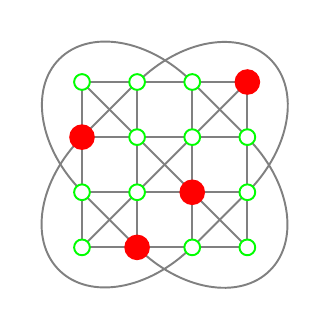
\begin{tikzpicture}  [scale=0.35]

\tikzstyle{every path}=[line width=0.7pt]

\newdimen\ms
\ms=0.1cm
\tikzstyle{s1}=[color=red,rectangle,inner sep=3.5]
\tikzstyle{c3}=[circle,inner sep={\ms/8},minimum size=4*\ms]
\tikzstyle{c2}=[circle,inner sep={\ms/8},minimum size=3*\ms]
\tikzstyle{c1}=[circle,inner sep={\ms/8},minimum size=2*\ms]
\tikzstyle{cs1}=[circle,inner sep={\ms/8},minimum size=1*\ms]

% Define positions of all observables

\coordinate (uuu) at ( 0,6);
\coordinate (uuv) at ( 2,6);
\coordinate (uvu) at ( 4,6);
\coordinate (uvv) at ( 6,6);
\coordinate (vuu) at ( 8,6);
\coordinate (vuv) at (10,6);
\coordinate (vvu) at (12,6);
\coordinate (vvv) at (14,6);

\coordinate (ucc) at ( 0,4);
\coordinate (vcc) at ( 2,4);
\coordinate (ucd) at ( 4,4);
\coordinate (vcd) at ( 6,4);
\coordinate (udc) at ( 8,4);
\coordinate (vdc) at (10,4);
\coordinate (udd) at (12,4);
\coordinate (vdd) at (14,4);

\coordinate (cuc) at ( 0,2);
\coordinate (cvc) at ( 2,2);
\coordinate (cud) at ( 4,2);
\coordinate (cvd) at ( 6,2);
\coordinate (duc) at ( 8,2);
\coordinate (dvc) at (10,2);
\coordinate (dud) at (12,2);
\coordinate (dvd) at (14,2);

\coordinate (ccu) at ( 0,0);
\coordinate (ccv) at ( 2,0);
\coordinate (cdu) at ( 4,0);
\coordinate (cdv) at ( 6,0);
\coordinate (dcu) at ( 8,0);
\coordinate (dcv) at (10,0);
\coordinate (ddu) at (12,0);
\coordinate (ddv) at (14,0);

% draw contexts

\draw [color=Gray] (ccu) -- (cdv);
\draw [color=Gray] (cuc) -- (cvd);
\draw [color=Gray] (ucc) -- (vcd);
\draw [color=Gray] (uuu) -- (uvv);

\draw [color=Gray] (uuu) -- (ccu);
\draw [color=Gray] (uuv) -- (ccv);
\draw [color=Gray] (uvu) -- (cdu);
\draw [color=Gray] (uvv) -- (cdv);

\draw [color=Gray] (uuu) -- (cdv);
\draw [color=Gray] (uvv) -- (ccu);

\draw [color=Gray] (uuv) -- (ucc);
\draw [color=Gray](cdu) -- (cvd);
\draw [rotate=225,color=Gray] (cvd) arc (90:270:4 and 2.82);
\draw[rotate=45,color=Gray] (ucc) arc (90:270:4 and 2.82);

\draw [color=Gray] (cuc) -- (ccv);
\draw [color=Gray] (uvu) -- (vcd);
\draw[rotate=315,color=Gray] (uvu) arc (90:270:4 and 2.82);
\draw[rotate=135,color=Gray] (ccv) arc (90:270:4 and 2.82);

%draw atoms

\draw (uuu) coordinate[c1,fill=white,draw=green];
\draw (uuv) coordinate[c1,fill=white,draw=green];
\draw (uvu) coordinate[c1,fill=white,draw=green];
\draw (uvv) coordinate[c2,fill=red,draw=red];


\draw (ucc) coordinate[c2,fill=red,draw=red];
\draw (vcc) coordinate[c1,fill=white,draw=green];
\draw (ucd) coordinate[c1,fill=white,draw=green];
\draw (vcd) coordinate[c1,fill=white,draw=green];

\draw (cuc) coordinate[c1,fill=white,draw=green];
\draw (cvc) coordinate[c1,fill=white,draw=green];
\draw (cud) coordinate[c2,fill=red,draw=red];
\draw (cvd) coordinate[c1,fill=white,draw=green];

\draw (ccu) coordinate[c1,fill=white,draw=green];
\draw (ccv) coordinate[c2,fill=red,draw=red];
\draw (cdu) coordinate[c1,fill=white,draw=green];
\draw (cdv) coordinate[c1,fill=white,draw=green];

\end{tikzpicture}
%
&
%
%%%%%%%%%%%%%%%%%%% 8
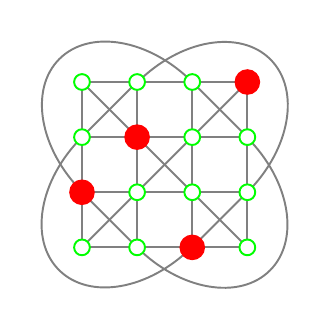
\begin{tikzpicture}  [scale=0.35]

\tikzstyle{every path}=[line width=0.7pt]

\newdimen\ms
\ms=0.1cm
\tikzstyle{s1}=[color=red,rectangle,inner sep=3.5]
\tikzstyle{c3}=[circle,inner sep={\ms/8},minimum size=4*\ms]
\tikzstyle{c2}=[circle,inner sep={\ms/8},minimum size=3*\ms]
\tikzstyle{c1}=[circle,inner sep={\ms/8},minimum size=2*\ms]
\tikzstyle{cs1}=[circle,inner sep={\ms/8},minimum size=1*\ms]

% Define positions of all observables

\coordinate (uuu) at ( 0,6);
\coordinate (uuv) at ( 2,6);
\coordinate (uvu) at ( 4,6);
\coordinate (uvv) at ( 6,6);
\coordinate (vuu) at ( 8,6);
\coordinate (vuv) at (10,6);
\coordinate (vvu) at (12,6);
\coordinate (vvv) at (14,6);

\coordinate (ucc) at ( 0,4);
\coordinate (vcc) at ( 2,4);
\coordinate (ucd) at ( 4,4);
\coordinate (vcd) at ( 6,4);
\coordinate (udc) at ( 8,4);
\coordinate (vdc) at (10,4);
\coordinate (udd) at (12,4);
\coordinate (vdd) at (14,4);

\coordinate (cuc) at ( 0,2);
\coordinate (cvc) at ( 2,2);
\coordinate (cud) at ( 4,2);
\coordinate (cvd) at ( 6,2);
\coordinate (duc) at ( 8,2);
\coordinate (dvc) at (10,2);
\coordinate (dud) at (12,2);
\coordinate (dvd) at (14,2);

\coordinate (ccu) at ( 0,0);
\coordinate (ccv) at ( 2,0);
\coordinate (cdu) at ( 4,0);
\coordinate (cdv) at ( 6,0);
\coordinate (dcu) at ( 8,0);
\coordinate (dcv) at (10,0);
\coordinate (ddu) at (12,0);
\coordinate (ddv) at (14,0);

% draw contexts

\draw [color=Gray] (ccu) -- (cdv);
\draw [color=Gray] (cuc) -- (cvd);
\draw [color=Gray] (ucc) -- (vcd);
\draw [color=Gray] (uuu) -- (uvv);

\draw [color=Gray] (uuu) -- (ccu);
\draw [color=Gray] (uuv) -- (ccv);
\draw [color=Gray] (uvu) -- (cdu);
\draw [color=Gray] (uvv) -- (cdv);

\draw [color=Gray] (uuu) -- (cdv);
\draw [color=Gray] (uvv) -- (ccu);

\draw [color=Gray] (uuv) -- (ucc);
\draw [color=Gray](cdu) -- (cvd);
\draw [rotate=225,color=Gray] (cvd) arc (90:270:4 and 2.82);
\draw[rotate=45,color=Gray] (ucc) arc (90:270:4 and 2.82);

\draw [color=Gray] (cuc) -- (ccv);
\draw [color=Gray] (uvu) -- (vcd);
\draw[rotate=315,color=Gray] (uvu) arc (90:270:4 and 2.82);
\draw[rotate=135,color=Gray] (ccv) arc (90:270:4 and 2.82);

%draw atoms

\draw (uuu) coordinate[c1,fill=white,draw=green];
\draw (uuv) coordinate[c1,fill=white,draw=green];
\draw (uvu) coordinate[c1,fill=white,draw=green];
\draw (uvv) coordinate[c2,fill=red,draw=red];


\draw (ucc) coordinate[c1,fill=white,draw=green];
\draw (vcc) coordinate[c2,fill=red,draw=red];
\draw (ucd) coordinate[c1,fill=white,draw=green];
\draw (vcd) coordinate[c1,fill=white,draw=green];

\draw (cuc) coordinate[c2,fill=red,draw=red];
\draw (cvc) coordinate[c1,fill=white,draw=green];
\draw (cud) coordinate[c1,fill=white,draw=green];
\draw (cvd) coordinate[c1,fill=white,draw=green];

\draw (ccu) coordinate[c1,fill=white,draw=green];
\draw (ccv) coordinate[c1,fill=white,draw=green];
\draw (cdu) coordinate[c2,fill=red,draw=red];
\draw (cdv) coordinate[c1,fill=white,draw=green];

\end{tikzpicture}
\end{tabular}
\end{center}
\caption{\label{2020-f-ghz-contextghz2vs}
Enumeration of the eight two-valued states of the GHZ logic.
}
\end{figure}

\begin{figure}[htb!]%[H]
\begin{center}
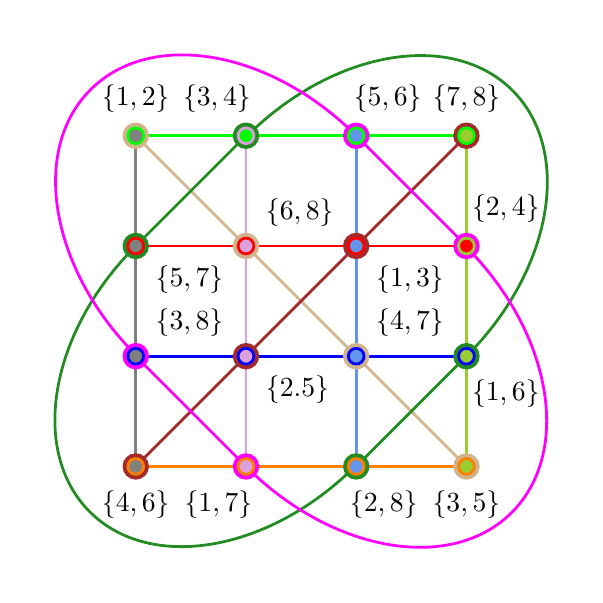
\begin{tikzpicture}  [scale=0.7]

\tikzstyle{every path}=[line width=1pt]

\newdimen\ms
\ms=0.1cm
\tikzstyle{s1}=[color=red,rectangle,inner sep=3.5]
\tikzstyle{c3}=[circle,inner sep={\ms/8},minimum size=4*\ms]
\tikzstyle{c2}=[circle,inner sep={\ms/8},minimum size=3*\ms]
\tikzstyle{c1}=[circle,inner sep={\ms/8},minimum size=2*\ms]
\tikzstyle{cs1}=[circle,inner sep={\ms/8},minimum size=1*\ms]


% Define positions of all observables

\coordinate (uuu) at ( 0,6);
\coordinate (uuv) at ( 2,6);
\coordinate (uvu) at ( 4,6);
\coordinate (uvv) at ( 6,6);
\coordinate (vuu) at ( 8,6);
\coordinate (vuv) at (10,6);
\coordinate (vvu) at (12,6);
\coordinate (vvv) at (14,6);


\coordinate (ucc) at ( 0,4);
\coordinate (vcc) at ( 2,4);
\coordinate (ucd) at ( 4,4);
\coordinate (vcd) at ( 6,4);
\coordinate (udc) at ( 8,4);
\coordinate (vdc) at (10,4);
\coordinate (udd) at (12,4);
\coordinate (vdd) at (14,4);

\coordinate (cuc) at ( 0,2);
\coordinate (cvc) at ( 2,2);
\coordinate (cud) at ( 4,2);
\coordinate (cvd) at ( 6,2);
\coordinate (duc) at ( 8,2);
\coordinate (dvc) at (10,2);
\coordinate (dud) at (12,2);
\coordinate (dvd) at (14,2);

\coordinate (ccu) at ( 0,0);
\coordinate (ccv) at ( 2,0);
\coordinate (cdu) at ( 4,0);
\coordinate (cdv) at ( 6,0);
\coordinate (dcu) at ( 8,0);
\coordinate (dcv) at (10,0);
\coordinate (ddu) at (12,0);
\coordinate (ddv) at (14,0);




% draw contexts

\draw [color=orange] (ccu) -- (cdv);
\draw [color=blue] (cuc) -- (cvd);
\draw [color=red] (ucc) -- (vcd);
\draw [color=green] (uuu) -- (uvv);

\draw [color=Gray] (uuu) -- (ccu);
\draw [color=Plum] (uuv) -- (ccv);
\draw [color=CornflowerBlue] (uvu) -- (cdu);
\draw [color=YellowGreen] (uvv) -- (cdv);


\draw [color=Tan] (uuu) -- (cdv);
\draw [color=Brown] (uvv) -- (ccu);


\draw [color=ForestGreen] (uuv) -- (ucc);
\draw [color=ForestGreen](cdu) -- (cvd);
\draw [rotate=225,color=ForestGreen] (cvd) arc (90:270:4 and 2.82);
\draw[rotate=45,color=ForestGreen] (ucc) arc (90:270:4 and 2.82);

\draw [color=Magenta] (cuc) -- (ccv);
\draw [color=Magenta] (uvu) -- (vcd);
\draw[rotate=315,color=Magenta] (uvu) arc (90:270:4 and 2.82);
\draw[rotate=135,color=Magenta] (ccv) arc (90:270:4 and 2.82);


%draw atoms




 \draw (uuu) coordinate[c2,fill=Tan,draw=Tan,label=above:{$\{1,2\}$}];
 \draw (uuu) coordinate[c1,fill=Gray,draw=green];
 \draw (uuv) coordinate[c2,fill=ForestGreen,draw=ForestGreen,label={[xshift=-3.7mm]90:$\{3,4\}$}];
 \draw (uuv) coordinate[c1,fill=green,draw=Plum];
 \draw (uvu) coordinate[c2,fill=Magenta,draw=Magenta,label={[xshift=+4mm]90:$\{5,6\}$}];
 \draw (uvu) coordinate[c1,fill=CornflowerBlue,draw=green];
 \draw (uvv) coordinate[c2,fill=Brown,draw=Brown,label=above:{$\{7,8\}$}];
 \draw (uvv) coordinate[c1,fill=YellowGreen,draw=green];


  % \draw (ucc) coordinate[c2,fill=ForestGreen,draw=ForestGreen,label={[xshift=-7.5mm,distance=0mm]90:$\{x_-  y_-  y_-\}$}];
   \draw (ucc) coordinate[c2,fill=ForestGreen,draw=ForestGreen,label=below right:{$\{5,7\}$}];
   \draw (ucc) coordinate[c1,fill=Gray,draw=red];
   \draw (vcc) coordinate[c2,fill=Tan,draw=Tan,label=above right:{$\{6,8\}$}];
   \draw (vcc) coordinate[c1,fill=Plum,draw=red];
   \draw (ucd) coordinate[c2,fill=Brown,draw=Brown,label=below right:{$\{1,3\}$}];
   \draw (ucd) coordinate[c1,fill=CornflowerBlue,draw=red];
  % \draw (vcd) coordinate[c2,fill=Magenta,draw=Magenta,label=above right:{$\{x_+  y_+  y_-\}$}];
   \draw (vcd) coordinate[c2,fill=Magenta,draw=Magenta,label={[xshift=+5mm,distance=10mm]90:$\{2,4\}$}];
   \draw (vcd) coordinate[c1,fill=red,draw=YellowGreen];

  \draw (cuc) coordinate[c2,fill=Magenta,draw=Magenta,label=above right:{$\{3,8\}$}];
  \draw (cuc) coordinate[c1,fill=Gray,draw=blue];
  \draw (cvc) coordinate[c2,fill=Brown,draw=Brown,label=below right:{$\{2.5\}$}];
  \draw (cvc) coordinate[c1,fill=Plum,draw=blue];
  \draw (cud) coordinate[c2,fill=Tan,draw=Tan,label=above right:{$\{4,7\}$}];
  \draw (cud) coordinate[c1,fill=CornflowerBlue,draw=blue];
  \draw (cvd) coordinate[c2,fill=ForestGreen,draw=ForestGreen,label={[xshift=+5mm,distance=10mm]270:$\{1,6\}$}];
  \draw (cvd) coordinate[c1,fill=YellowGreen,draw=blue];

\draw (ccu) coordinate[c2,fill=Brown,draw=Brown,label=below:{$\{4,6\}$}];
\draw (ccu) coordinate[c1,fill=Gray,draw=orange];
\draw (ccv) coordinate[c2,fill=Magenta,draw=Magenta,label={[xshift=-3.5mm]270:$\{1,7\}$}];
\draw (ccv) coordinate[c1,fill=Plum,draw=orange];
\draw (cdu) coordinate[c2,fill=ForestGreen,draw=ForestGreen,label={[xshift=+3.5mm]270:$\{2,8\}$}];
\draw (cdu) coordinate[c1,fill=CornflowerBlue,draw=orange];
\draw (cdv) coordinate[c2,fill=Tan,draw=Tan,label=below:{$\{3,5\}$}];
\draw (cdv) coordinate[c1,fill=YellowGreen,draw=orange];



\end{tikzpicture}
\end{center}
\caption{\label{2020-f-ghz-contextpl}
Hypergraphs representing  the 12 tightly intertwined GHZ contexts in a partition logic representation.
}
\end{figure}

From this partition logic
\begin{equation}
\begin{aligned}
&\{
\{1,2\},\{3,4\},\{5,6\},\{7,8\}
\},\\
&\{
\{5,7\},\{6,8\},\{1,3\},\{2,4\}
\},\\
&\{
\{3,8\},\{2,5\},\{4,7\},\{1,6\}
\},\\
&\{
\{4,6\},\{1,7\},\{2,8\},\{3,5\}
\},\\
&\{
\{1,2\},\{6,8\},\{4,7\},\{3,5\}
\},\\
&\{
\{7,8\},\{1,3\},\{2,5\},\{4,6\}
\},\\
&\{
\{5,6\},\{2,4\},\{3,8\},\{1,7\}
\},\\
&\{
\{3,4\},\{5,7\},\{1,6\},\{2,8\}
\}
\end{aligned}
\label{2020-ghz-e-pl}
\end{equation}
one can immediately derive a classical winning strategy for the GHZ game which is context dependent and requires knowledge of the configuration or context involved.
All that is needed is the identification of the respective vertices in the original configuration and the partition logic
(any other variation within the horizontal contexts would also suffice);
e.g.,
$\{1,2\} \mapsto x_+x_+x_+$,
$\{3,4\} \mapsto x_+x_-x_-$, $\ldots$,
$\{2,8\} \mapsto y_+y_+x_-$.
Then the associated generalized urn model reproduces the quantum mechanical predictions such as expectation values and distributions of oder one, two, and three.

A typical experimental run would consist of a (generalized urn ``loaded'' with (triples of identical) balls of eight types and four colors, associated with
the ward's potential choice of configurations or contexts.
Upon drawing such a ball triple the prisoners take their share of the triple--exactly one ball from the triple--and, in accordance with the ward's choice,
read the pairs of numbers (from one to eight) in that respective color. Their choice must then be their position of the identified answer.
More explicitly, if they read ``$3,4$'' in the color associated with the first context,
the first prisoner writes or shouts ``$+$''1,
the second prisoner writes or shouts ``$-$''1,
the third prisoner writes or shouts ``$-$''1.


############################################################

xp = {1,1}; xm = {1,-1}; yp = {1,I}; ym = {1,-I};

contexts = {};

con1 = {
{
Flatten[ KroneckerProduct[ xp , Flatten[ KroneckerProduct[ xp , xp ]]]],
Flatten[ KroneckerProduct[ xp , Flatten[ KroneckerProduct[ xm , xm ]]]],
Flatten[ KroneckerProduct[ xm , Flatten[ KroneckerProduct[ xp , xm ]]]],
Flatten[ KroneckerProduct[ xm , Flatten[ KroneckerProduct[ xm , xp ]]]]},
{
Flatten[ KroneckerProduct[ xm , Flatten[ KroneckerProduct[ ym , ym ]]]],
Flatten[ KroneckerProduct[ xm , Flatten[ KroneckerProduct[ yp , yp ]]]],
Flatten[ KroneckerProduct[ xp , Flatten[ KroneckerProduct[ ym , yp ]]]],
Flatten[ KroneckerProduct[ xp , Flatten[ KroneckerProduct[ yp , ym ]]]]},
{
Flatten[ KroneckerProduct[ ym , Flatten[ KroneckerProduct[ xm , ym ]]]],
Flatten[ KroneckerProduct[ ym , Flatten[ KroneckerProduct[ xp , yp ]]]],
Flatten[ KroneckerProduct[ yp , Flatten[ KroneckerProduct[ xm , yp ]]]],
Flatten[ KroneckerProduct[ yp , Flatten[ KroneckerProduct[ xp , ym ]]]]},
{
Flatten[ KroneckerProduct[ ym , Flatten[ KroneckerProduct[ ym , xm ]]]],
Flatten[ KroneckerProduct[ ym , Flatten[ KroneckerProduct[ yp , xp ]]]],
Flatten[ KroneckerProduct[ yp , Flatten[ KroneckerProduct[ ym , xp ]]]],
Flatten[ KroneckerProduct[ yp , Flatten[ KroneckerProduct[ yp , xm ]]]]
}} ;


TensorProductVec[x_, y_] :=
  Flatten[Table[
    x[[i]] y[[j]], {i, 1, Length[x]}, {j, 1, Length[y]}]];

con2 = {
{
TensorProductVec[ xp , TensorProductVec[ xp , xp ]],
TensorProductVec[ xp , TensorProductVec[ xm , xm ]],
TensorProductVec[ xm , TensorProductVec[ xp , xm ]],
TensorProductVec[ xm , TensorProductVec[ xm , xp ]]},
{
TensorProductVec[ xm , TensorProductVec[ ym , ym ]],
TensorProductVec[ xm , TensorProductVec[ yp , yp ]],
TensorProductVec[ xp , TensorProductVec[ ym , yp ]],
TensorProductVec[ xp , TensorProductVec[ yp , ym ]]},
{
TensorProductVec[ ym , TensorProductVec[ xm , ym ]],
TensorProductVec[ ym , TensorProductVec[ xp , yp ]],
TensorProductVec[ yp , TensorProductVec[ xm , yp ]],
TensorProductVec[ yp , TensorProductVec[ xp , ym ]]},
{
TensorProductVec[ ym , TensorProductVec[ ym , xm ]],
TensorProductVec[ ym , TensorProductVec[ yp , xp ]],
TensorProductVec[ yp , TensorProductVec[ ym , xp ]],
TensorProductVec[ yp , TensorProductVec[ yp , xm ]]
}} ;

con1 == con2

MatrixForm[Table[ con1[[1,i]] . Conjugate[ con1[[1,j]] ], {i,4},{j,4}]]

MatrixForm[Table[ con1[[2,i]] . Conjugate[ con1[[2,j]] ], {i,4},{j,4}]]

MatrixForm[Table[ con1[[3,i]] . Conjugate[ con1[[3,j]] ], {i,4},{j,4}]]

MatrixForm[Table[ con1[[4,i]] . Conjugate[ con1[[4,j]] ], {i,4},{j,4}]]

contexts = {};

Do[
Do[
Do[
Do[

If[ con1[[1,i1]] .  (* WRONG NOT TO Conjugate[ *)  con1[[2,i2]] (* ] *)  == 0,
If[ con1[[1,i1]] .  (* WRONG NOT TO Conjugate[ *)  con1[[3,i3]] (* ] *)  == 0,
If[ con1[[1,i1]] .  (* WRONG NOT TO Conjugate[ *)  con1[[4,i4]] (* ] *)  == 0,

If[ con1[[2,i2]] .  (* WRONG NOT TO Conjugate[ *)  con1[[3,i3]] (* ] *)  == 0,
If[ con1[[2,i2]] .  (* WRONG NOT TO Conjugate[ *)  con1[[4,i4]] (* ] *)  == 0,

If[ con1[[3,i3]] .  (* WRONG NOT TO Conjugate[ *)  con1[[4,i4]] (* ] *)  == 0,  AppendTo[contexts, {i1, i2, i3, i4}]
]]]]]]

,{i4,4}]
,{i3,4}]
,{i2,4}]
,{i1,4}]

contexts

{{1, 1, 1, 1}, {1, 2, 3, 4}, {2, 1, 4, 3}, {2, 2, 2, 2}, {3, 3, 3, 3}, {3, 4, 1, 2}, {4, 3, 2, 1}, {4, 4, 4, 4}}
